\documentclass[11pt,a4paper]{article}
\usepackage[T1]{fontenc}
\usepackage[utf8]{inputenc}
\usepackage{lmodern}
\usepackage{microtype,amsmath,amssymb,amsthm,mathtools}
\usepackage{booktabs,array,longtable,graphicx,float,xcolor}
\usepackage[margin=2.05cm]{geometry}
\usepackage{enumitem,fancyhdr,hyperref}
\hypersetup{unicode=true,colorlinks=true,linkcolor=blue!45!black,urlcolor=blue!55!black,
 pdftitle={FIN ST447--ST461: Global Transition, Exact Degree-Six Relations, and Adaptive Infrared Continuation},
 pdfauthor={Krzysztof Żuchowski},
 pdfsubject={Finite analytical and computational continuation of FIN},
 pdfkeywords={FIN, strict kernel, entropy, global phase transition, invariant theory, Krawczyk, infrared continuation}}
\pagestyle{fancy}\fancyhf{}\lhead{FIN ST447--ST461}\rhead{Release 10.87}\cfoot{\thepage}
\setlength{\headheight}{14pt}
\newcommand{\Proven}{\textcolor{green!38!black}{\textbf{[PROVEN]}}}
\newcommand{\Evidence}{\textcolor{orange!80!black}{\textbf{[STRONG NUMERICAL EVIDENCE]}}}
\newcommand{\Partial}{\textcolor{orange!80!black}{\textbf{[PARTIAL]}}}
\newcommand{\Blocked}{\textcolor{red!65!black}{\textbf{[BLOCKED]}}}
\newtheorem{theorem}{Theorem}
\newtheorem{proposition}{Proposition}
\newtheorem{corollary}{Corollary}

\title{\textbf{FIN ST447--ST461}\\[3pt]
Global Gain Transition, Exact Degree-Six Invariant Relations,\\
and Adaptive Infrared Continuation\\[6pt]
\large Release 10.87}
\author{Krzysztof Żuchowski\\
\small Independent Researcher --- Fractal Information Theory Project\\
\small ORCID: 0009-0002-0909-3613}
\date{14 August 2026}

\begin{document}
\maketitle

\begin{abstract}
Programs ST447--ST461 continue the local analytical and computational FIN
research program after Release 10.86.  The principal result is the first
computer-assisted global lower certificate close to the previously isolated
reflection-even coexistence branch.  For the supplied dimensionless family
\[
 V_g(p)=D(p\Vert u)-\frac g2(p-u)^TA(p-u),\qquad p\in\Delta_{11},
\]
the uniform state is now proved to be the unique global minimizer for every
$0\le g\le2.8934$.  A previously certified nonuniform competitor has negative
value at $g=2.9024964917477667$.  Consequently a first global transition exists
in the interval
\[
 [2.8934,\,2.9024964917477667],
\]
of width $0.0090964917477665$.  The identity of the first competing orbit and
transition uniqueness remain open; in particular, the local branch crossing
is not silently promoted to the global transition.

The invariant-algebra result is exact.  A two-prime calculation reconstructs
sixteen primitive integer relations among the 326 declared decomposable
degree-six invariants.  Direct characteristic-zero polynomial division by
$x_0+\cdots+x_{11}$ verifies every relation.  Together with a nonzero modular
rank-310 minor, this proves characteristic-zero decomposable rank $310$ and
primitive quotient dimension $365-310=55$.  At degree eight, a projective
incidence census checks every triple made collinear by two independent finite
field projections against the complete evaluation matrix.  No rational
syzygy of support at most three exists; the forced relation basis must begin
at support four or larger.

The compactified infrared branch is continued by 28 overlapping parametric
Krawczyk cells from $b=0.017$ to $b=0.1$, with independently certified common
root boxes at every interface.  Combined with ST437, this proves one connected
locally unique component from $b=0$ through $0.1$, retaining ordering,
orientation, and local Brouwer degree $-1$.  It does not count roots outside
the chain.  Secondary programs expose two useful negative results: five
synthetic design exchanges improve in-design E/A conditioning but worsen
frozen holdout leverage, and larger Ulam grids invalidate the earlier visual
plateau interpretation.  No program derives the gain, supplies a
nonpremise selector, fixes dimensional units, transfers legacy physical roles,
or adds independent empirical evidence.
\end{abstract}

\tableofcontents
\newpage

\section{Scope, source packet, and nonclaims}

The audited tracked baseline is Git commit
\texttt{bb540a767e210a5a3bf816e4868e7bcefbac3872}, supplemented by the local
ST417--ST446 executable packets listed in Section~\ref{sec:repro}.  The strict
finite operator is
\begin{equation}\label{eq:A}
 A=sI-W,\qquad W_{xx}=0,\qquad
 W_{xy}=\frac{\cos(0.18575d(x,y)+0.16250)}{1+d(x,y)^{9/5}}\quad(x\ne y),
\end{equation}
on $\mathbb Z_{12}$, with off-diagonal row sum
$s=1.660307278766099\ldots$.  Every quantity in this report is
dimensionless.

The legacy ontological kernel remains an intermediate bridge kernel; it is not
silently identified with \eqref{eq:A}.  No legacy claim concerning
electroweak parameters, electromagnetic coupling, a gravity hierarchy,
Planck scales, or matter generation is transferred.  The project ontology is
retained only as context: the nadsoliton itself is primordial fractal
information in a solitonic state, with no informational substrate below it,
and with preferred internal order nadsoliton $\to$ light $\to$ matter $\to$
emergent observer.

A global orbit is not a selector.  QW-2191 remains open.  A theorem conditional
on $g$ does not source $g$.  The infrared variables are names in a
dimensionless optimization fixture and are not physical wavelengths or
energies.  Local computation is not external validation and does not establish
a Theory of Everything.

\section{Executive result ledger}
\small
\begin{longtable}{>{\raggedright\arraybackslash}p{.075\textwidth}>{\raggedright\arraybackslash}p{.18\textwidth}>{\raggedright\arraybackslash}p{.64\textwidth}}
\toprule Program&Status&Result\\\midrule\endhead
ST447&\Proven{}&No rational degree-eight relation supported on one, two, or three of the 2028 declared candidates.  The forced relation basis remains unknown.\\
ST448&\Proven{}&The uniform state is the unique global minimizer for every supplied $0\le g\le2.8934$.\\
ST449&\Proven{}&A first global change exists in $[2.8934,2.9024964917477667]$; branch identity and uniqueness are open.\\
ST450&\Proven{} limited&The partial Morse polynomial factors as $1+(1+t)(12+30t)$ and satisfies the strong Morse condition.  This does not prove completeness.\\
ST451&\Proven{} local&Each certified index-one saddle has a stabilizer-invariant one-dimensional unstable eigenspace.  Heteroclinic endpoints remain numerical.\\
ST452&\Proven{} local&Twenty-eight Krawczyk cells and 28 certified interface boxes continue one component through $b=0.1$.\\
ST453&\Proven{} local&The component has $y_1<y_2<y_3$, $0<a<1$, $T>1$, negative Jacobian orientation, and local degree $-1$.\\
ST454&\Proven{}&Sixteen exact integer relations close the characteristic-zero degree-six rank at $310$ and quotient dimension at $55$.\\
ST455&\Evidence{} / falsified robustness&Five exchanges improve E by $17.20\%$ and A by $15.87\%$, but worsen frozen holdout leverage; robustness is rejected.\\
ST456&\Evidence{} / caution&Grids 71 and 81 show continued Ulam-ratio drift.  No infinite-dimensional two-sided transfer-gap bracket exists.\\
ST457&\Proven{} conditional&The conservative scalar ISS architecture has a unique optimal radius $1.9360740\times10^{-6}$.\\
ST458&\Blocked&Current sign-aware and absolute-value relaxations do not close the rank-seven global problem.\\
ST459&\Blocked&No internal strict source of $g$ is exported.\\
ST460&\Blocked&No nonpremise selector is exported; QW-2191 remains open.\\
ST461&\Blocked&No independent referee, laboratory record, custody chain, or held-out empirical datum is added.\\
\bottomrule
\end{longtable}
\normalsize

\section{ST448--ST449: the first narrow global-transition theorem}

Let $u_i=1/12$, $q=p-u$, and
\begin{equation}\label{eq:V}
 D(p\Vert u)=\sum_{i=0}^{11}p_i\log(12p_i),\qquad
 V_g(p)=D(p\Vert u)-\frac g2q^TAq.
\end{equation}
Because $A$ is positive semidefinite and has constants as its kernel, $V_g(p)$
is nonincreasing in $g$ for each fixed nonuniform $p$.

\subsection{A separable entropy-curvature lemma}

Put $r=1/12$ and
\begin{equation}\label{eq:h}
 h(m)=\frac{m\log(12m)-(m-r)}{(m-r)^2}.
\end{equation}
Elementary differentiation shows that
\[
 \frac{x\log(12x)-(x-r)}{(x-r)^2}\ge h(m)
 \quad\text{for }0\le x\le m,\quad m>r.
\]
The removable value at $x=r$ is $6$.  Summing the scalar inequalities and
using $\sum_i(p_i-r)=0$ yields
\begin{equation}\label{eq:sep}
 D(p\Vert u)\ge h(m)\lVert p-u\rVert_2^2
 \quad\text{whenever }\max_i p_i\le m.
\end{equation}
Since $q^TAq\le\lambda_{\max}(A)\lVert q\rVert^2$, the sector is strictly
positive if $h(m)>g\lambda_{\max}/2$.

At $g=2.8934$ and
\[
 \lambda_{\max}(A)=2.342182041146300\ldots,
 \qquad m_0=0.33426904850345385,
\]
the paid scalar margin is
\[
 h(m_0)-\frac{g\lambda_{\max}}2
 =4.949286539379649\times10^{-4}>0.
\]
Thus the complete low-maximum sector is closed analytically.

\subsection{The complementary two-variable cover}

Select a largest coordinate and write
\[
 p_0=1-t,\qquad p_j=t y_j,\qquad
 \sum_{j=1}^{11}y_j=1,\qquad \rho=\sum_{j=1}^{11}y_j^2.
\]
The high sector is the rectangle
\[
 0\le t\le1-m_0,\qquad 1/11\le\rho\le1.
\]
At fixed $\rho$, the entropy minimum is bounded by the one-large,
ten-equal extremal distribution.  For the quadratic part write $W=sI-A$ and
let $R=W_{\{1,\dots,11\}}$.  With $\bar y=\mathbf 1/11$, $P=I-J/11$, the
remainder obeys two simultaneous lower bounds:
\begin{align}
 y^TRy&\ge w_{\min}(1-\rho),\\
 y^TRy&\ge c_0-2\ell\sqrt{\rho-1/11}
                +e_{\min}(\rho-1/11),\label{eq:Rbound}
\end{align}
where
\begin{align*}
 c_0&=0.13721547758397512,&
 \ell&=0.048732847203611034,\\
 e_{\min}&=-0.6703735434067706,&
 w_{\min}&=0.011070817321442113.
\end{align*}
The center-to-remainder term uses a feasible SOCP-dual water-fill lower bound,
not an unconstrained eigenvalue guess.

A $100\times100$ initial grid was recursively split only where its outward-paid
lower bound was nonpositive.  The completed tree contains 224,626 accepted
leaves, 71,542 refined nodes, and maximum depth nine.  The smallest lower
bound after a total $10^{-10}$ IEEE/libm payment per evaluated cell is
\begin{equation}\label{eq:globalmargin}
 2.437168031224723\times10^{-9}>0.
\end{equation}
It occurs in a depth-eight cell near
$t\in[0.10919548,0.10922149]$ and
$\rho\in[0.11697443,0.11700995]$.

\begin{theorem}[Uniform global regime]\label{thm:uniform}
For the supplied strict operator \eqref{eq:A} and every supplied
$0\le g\le2.8934$, the uniform probability is the unique global minimizer of
$V_g$ on the complete simplex.
\end{theorem}

The proof joins \eqref{eq:sep} and the complementary cover.  Strictness holds
in both sectors away from $u$, and monotonicity propagates the $g=2.8934$
certificate to smaller nonnegative gains.

\subsection{Existence, but not identity, of the first transition}

For $p\ne u$, the equal-value gain is
\begin{equation}\label{eq:ratio}
 R(p)=\frac{2D(p\Vert u)}{(p-u)^TA(p-u)}.
\end{equation}
Near $u$ its directional lower limit is
\[
 \liminf_{p\to u}R(p)\ge\frac{12}{\lambda_{\max}(A)}
 =5.123427551398616,
\]
well above the relevant interval.  Hence the infimum is attained away from
$u$ on a compact subset.  Theorem~\ref{thm:uniform} supplies the lower bound.
The ST342 interval state has certified negative value at
$g=2.9024964917477667$, supplying the upper bound.

\begin{theorem}[First global-transition bracket]
The first supplied gain at which a nonuniform state can match or beat the
uniform state exists and lies in
\[
 \boxed{[2.8934,\;2.9024964917477667]}.
\]
The bracket width is $0.0090964917477665$.
\end{theorem}

\begin{figure}[H]\centering
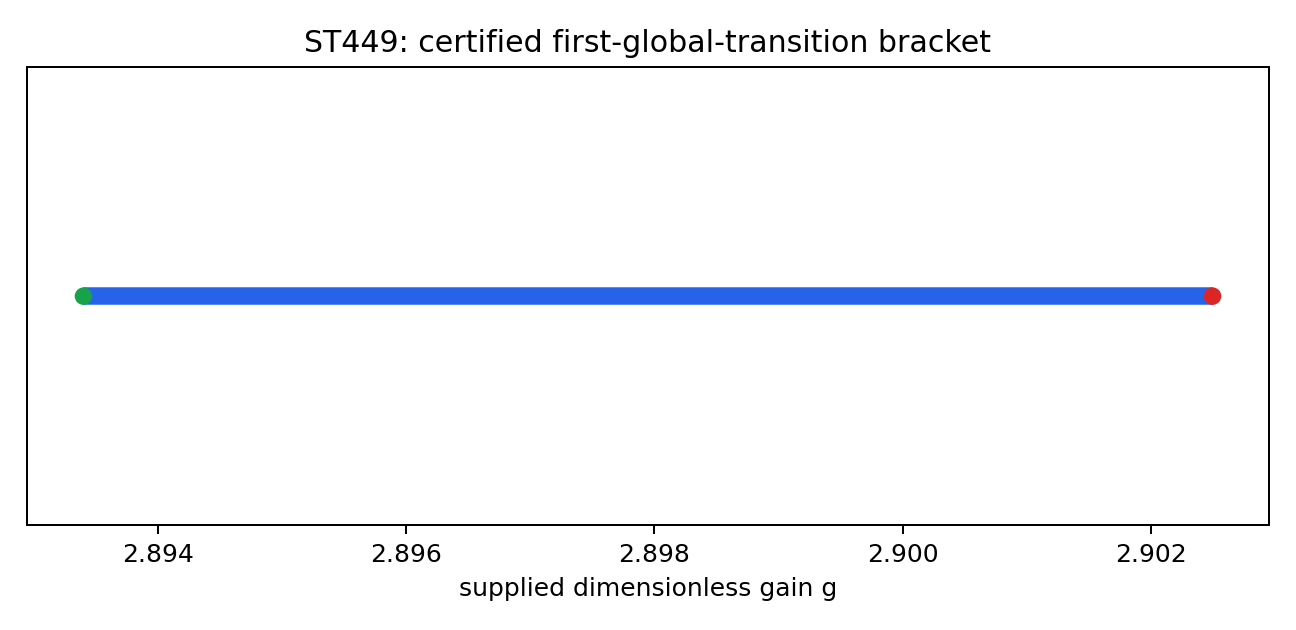
\includegraphics[width=.78\textwidth]{FIN_ST447_ST461_Figures/st449_global_transition_bracket.png}
\caption{The certified lower regime and a certified negative competitor bound
the first global transition.  The figure does not identify the first orbit.}
\end{figure}

The strongest falsification safeguard is explicit: the reflection-even
stationary branch crosses zero transversely near the upper endpoint, but an
unknown third orbit could realize \eqref{eq:ratio} earlier.  Neither global
branch identity nor uniqueness is claimed.

\section{ST447 and ST454: exact invariant-algebra advances}

\subsection{Degree eight: no support-three relation}

The degree-eight candidate list has
\[
 \binom{9}{4}+\binom{7}{2}32+\binom{33}{2}+6\cdot117=2028
\]
columns, while the Molien dimension is $1892$, forcing nullity at least $136$.
Release 10.86 excluded support one and two.  ST447 projects the full 64-row
evaluation matrix to a collision-free projective plane over each of
$\mathbb F_{1000003}$ and $\mathbb F_{1000033}$.  Every projected collinear
triple is then checked in the original 64-row matrix; projection may create a
false candidate but cannot hide a true dependency.

The two audits enumerate all 2,055,378 column pairs.  They respectively send
1,337 and 1,390 candidate triples to the full-matrix rank test.  None has rank
below three.

\begin{proposition}
No rational relation among the declared degree-eight candidates has support
at most three.  Therefore every one of the at least 136 forced relations has
support at least four.
\end{proposition}

This is an exclusion theorem, not an explicit relation basis.

\subsection{Degree six: exact closure in characteristic zero}

The 326 decomposable candidates are
\[
 56\;(q^3)\; +\;192\;(qP_4)\; +\;78\;(D_3D_3).
\]
Column elimination at both declared primes gives rank $310$ and the identical
set of 16 dependent pivot columns.  Chinese remaindering followed by rational
reconstruction yields 16 primitive integer vectors.  Their supports range
from $113$ to $311$; the largest coefficient appearing in the packet is
$512016$.

Modular agreement alone would be evidence, not a characteristic-zero upper
rank theorem.  Therefore every lifted combination was constructed as an exact
integer polynomial and divided synthetically by
\[
 L=x_0+x_1+\cdots+x_{11}.
\]
All sixteen remainders are literally the empty polynomial.  The relations are
independent because the column-elimination form has distinct leading
dependent columns.  Thus rank over $\mathbb Q$ is at most $310$.  Conversely,
the nonzero modular rank-310 minor is a nonzero integer minor, so the rational
rank is at least $310$.

\begin{theorem}[Exact degree-six presentation rank]
In the mean-zero quotient, the declared decomposable degree-six family has
characteristic-zero rank exactly $310$ and a sixteen-dimensional relation
kernel.  Since the full invariant dimension is $365$, the primitive quotient
dimension is exactly
\[
 365-310=55.
\]
\end{theorem}

The complete vectors, candidate descriptors, two-prime residues, and exact
division audits are stored separately in
\texttt{FIN\_ST454\_Degree6\_Integer\_Relations.json}.  The result closes the
ST439 interval $[39,55]$ at its upper endpoint.  It does not solve the
degree-eight presentation.

\section{ST450--ST453: topology and the adaptive infrared chain}

\subsection{What the partial Morse polynomial does and does not prove}

The certified nonexhaustive stationary census from ST435 has
\[
 M_{\rm partial}(t)=13+42t+30t^2.
\]
ST450 records the stronger identity
\begin{equation}\label{eq:Morse}
 M_{\rm partial}(t)=1+(1+t)(12+30t).
\end{equation}
The correction polynomial has nonnegative coefficients, so the census obeys
the strong Morse-polynomial condition for a contractible simplex, not merely
the Euler check at $t=-1$.

This is still not completeness: additional critical points may contribute
another $(1+t)R(t)$ with nonnegative coefficients.  Boundary strata are not
covered.  ST451 proves a local symmetry statement only.  At each of four
certified index-one representatives, the Hessian commutes with the exact
stabilizer; simplicity of the negative eigenvalue makes its unstable line a
one-dimensional real stabilizer representation.  The two global endpoints of
that line remain numerical and no Conley connection matrix is promoted.

\subsection{Removing the common-box bottleneck}

The prior compactification uses $b=1/y_3$ and $a=bc$.  A single common box was
certified only through $b=0.017$.  ST452 replaces it by direct interval
equations on cells $[b_-,b_+]$ with $b_->0$.  The apparently ill-conditioned
third stationarity equation is evaluated algebraically as
\[
 \frac{2c}{1+e^{-1/b}}+
 \frac{2T(1-bc)b^{-1}e^{-(T-1)/b}}{1+e^{-T/b}}-\nu=0.
\]
For the tail integral, the rigorous inequalities
\[
 \frac{e^{-y}}{y+1}\le E_1(y)\le\frac{e^{-y}}{y},\qquad y>0,
\]
avoid catastrophic interval cancellation.

Twenty-eight width-$0.003$ or smaller parametric Krawczyk cells cover
$[0.017,0.1]$.  Their minimum inclusion margin is
$1.8024\times10^{-7}$ and their maximum weighted contraction is $0.047294$.
At every one of the 28 interfaces, including $b=0.017$, a separate tiny
parametric Krawczyk box is contained in both neighboring boxes.  This proves
that the locally unique roots belong to one connected component rather than
merely producing a list of unrelated local roots.

\begin{theorem}[Connected regularized IR component]
Together with ST437, the displayed Krawczyk chain proves one locally unique
root component for every $b\in[0,0.1]$.  Throughout the new part,
\[
 y_1<0.028634<3.78868<y_2<3.87733<10\le y_3,
\]
$a\in[0.00059487,0.00367448]$, $T>1$, every Jacobian has negative
orientation, and the local Brouwer degree is $-1$.
\end{theorem}

\begin{figure}[H]\centering
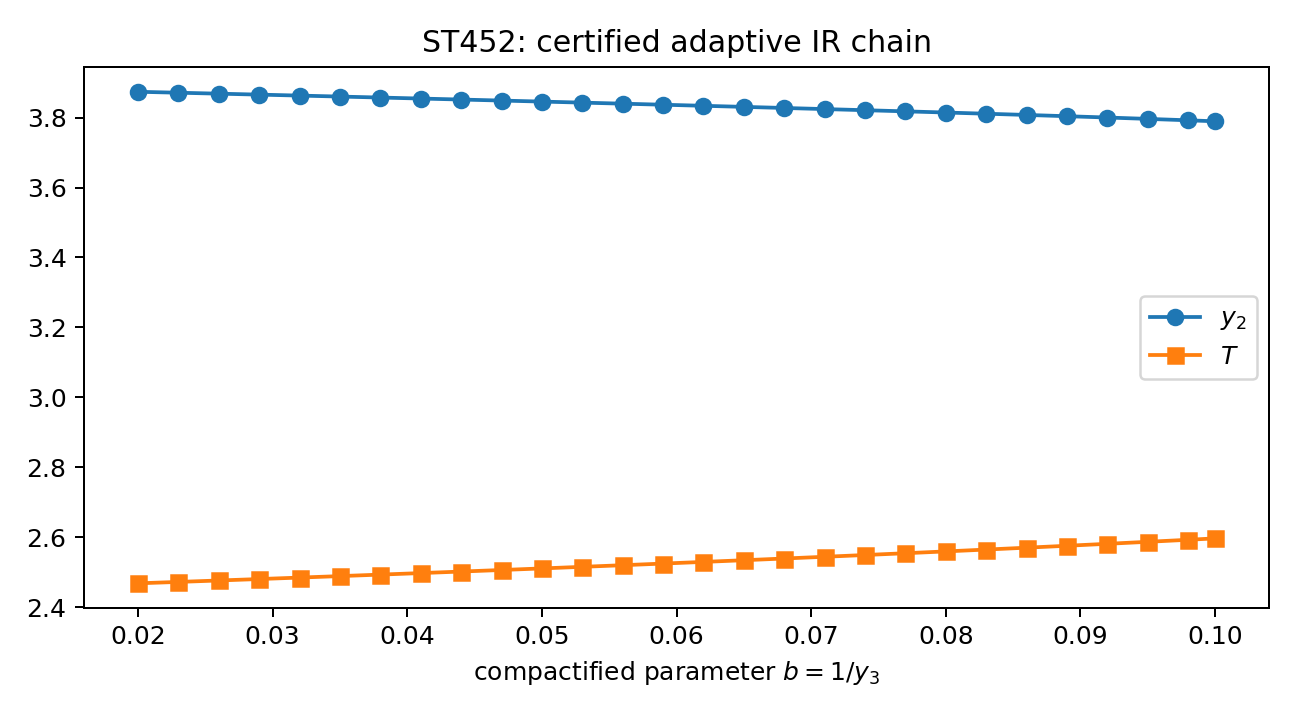
\includegraphics[width=.8\textwidth]{FIN_ST447_ST461_Figures/st452_ir_chain.png}
\caption{Centers from the certified adaptive cells.  Lines are visual guides;
the theorem is carried by the Krawczyk boxes and certified interface links.}
\end{figure}

No full complement cover has been performed.  Disconnected positive roots
outside the displayed boxes remain possible.

\section{ST455--ST458: adversarial secondary results}

\subsection{Synthetic design: training improves, holdout worsens}

Five weakest-direction row exchanges on the frozen 1,800-point synthetic pool
raise the smallest singular value by a factor $1.17195$ and improve the
A-trace-inverse criterion by a factor $1.15870$.  That looks favorable if only
the selected 500 rows are scored.  A frozen 1,295-row holdout reverses the
interpretation:
\begin{center}
\begin{tabular}{lrr}
\toprule&baseline&after five exchanges\\\midrule
maximum leverage&3.58940&4.02581\\
95th percentile leverage&2.78823&2.85715\\\bottomrule
\end{tabular}
\end{center}
The procedure overfits its in-design weakest direction.  ST455 therefore
rejects the word ``robust'' for this exchange rule.  No apparatus calibration
is inferred from a synthetic pool.

\subsection{Transfer sequence: the apparent plateau was premature}

Extending the Ulam sequence from grids $21,31,41,51,61$ to $71,81$ gives
\[
 \frac{|\lambda_2|}{|\lambda_1|}=0.5957361291\quad(n=71),\qquad
 0.5957254767\quad(n=81).
\]
The new last-two spread $1.0652\times10^{-5}$ is larger, not smaller, than the
previous $2.7505\times10^{-6}$ spread.  The sequence remains monotone over the
tested grids, but visual stabilization is not an error theorem.  Only the
coarser analytic Birkhoff bound remains certified.

\begin{figure}[H]\centering
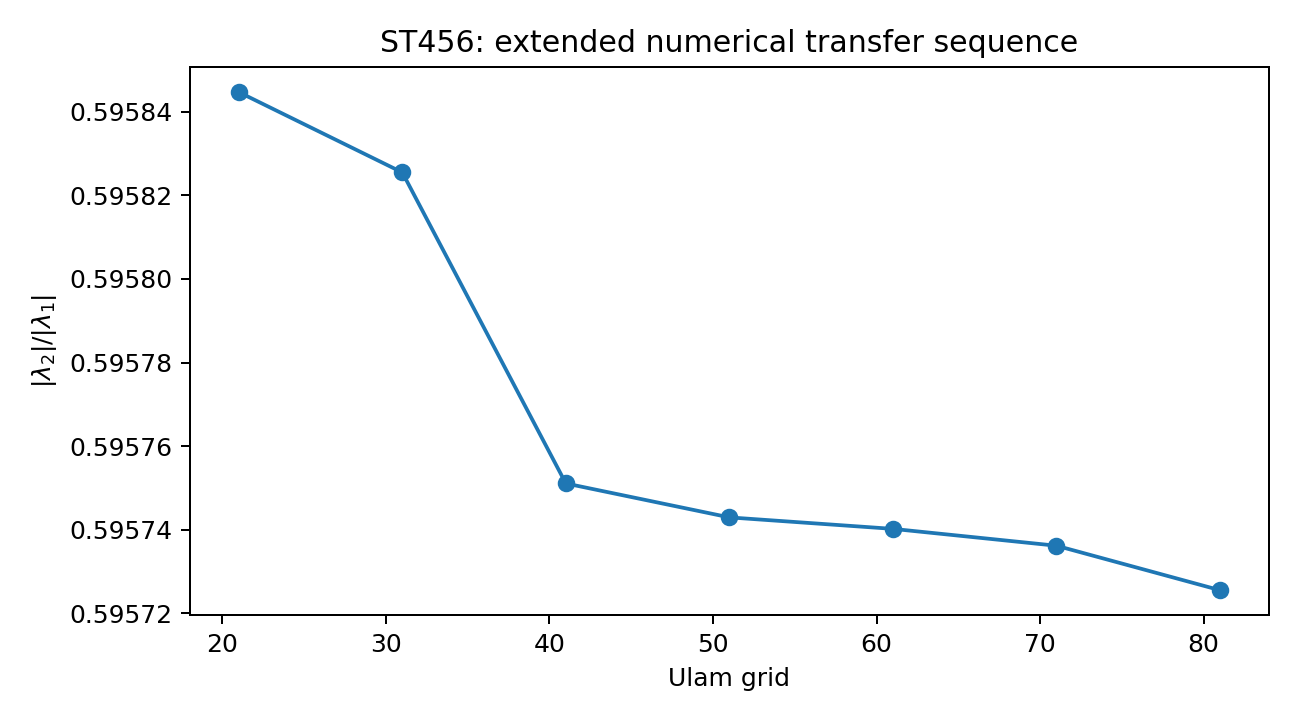
\includegraphics[width=.78\textwidth]{FIN_ST447_ST461_Figures/st456_ulam_extension.png}
\caption{The numerical ratio continues to drift.  No infinite-dimensional
two-sided spectral-gap bracket is claimed.}
\end{figure}

\subsection{A sharp result inside one conservative ISS architecture}

For the previously certified local minimum, the scalar estimate is
\[
 \mu(R)=\mu_0-\frac{R}{(p_{\min}-R)^2},\qquad
 \varepsilon(R)=\frac{R\mu(R)}2.
\]
It has a unique interior optimum satisfying
\[
 \mu_0=\frac{2Rp_{\min}}{(p_{\min}-R)^3}.
\]
With $p_{\min}=0.0002146796264$ and
$\mu_0=86.33235115$, the result is
\[
 R_*=1.9360740425\times10^{-6},\quad
 \mu(R_*)=43.55546688,\quad
 \varepsilon_*=4.2163304418\times10^{-5}.
\]
This proves optimality only within the stated Hessian-variation formula, not a
global basin and not a physical noise law.

ST458 also retains an honest stop.  The rank-seven mediator has 24 positive
and 42 negative off-diagonal pairs.  Positive-weight water filling does not
apply, while spectral and absolute-row-sum bounds are too weak at $g=4$.
No sign-aware global SDP certificate is available, so the known local
rank-seven state is not promoted to a global minimizer.

\section{Falsification ledger and scientific interpretation}

\begin{longtable}{>{\raggedright\arraybackslash}p{.27\textwidth}>{\raggedright\arraybackslash}p{.29\textwidth}>{\raggedright\arraybackslash}p{.35\textwidth}}
\toprule Claim tested&What survived&What failed or remains open\\\midrule\endhead
The local branch crossing is the first global transition&A first transition is now tightly bracketed.&No theorem identifies the attaining orbit; a third competitor is admissible.\\
Degree-six modular rank is characteristic-zero rank&Sixteen lifted relations verify exactly and close rank $310$.&The same closure has not been achieved at degree eight.\\
Low-support degree-eight relations should be easy to find&Support one, two, and three are exactly excluded.&The at-least-136-dimensional kernel must be denser; no basis is known.\\
The IR branch stops near $b=0.017$&The stop was a common-box artifact; adaptive boxes reach $0.1$.&A global root count and further continuation are open.\\
More design exchanges improve robustness&In-design E and A metrics improve.&Frozen holdout leverage worsens; robustness is falsified.\\
The Ulam ratio had stabilized&The tested sequence remains orderly and monotone.&New grids reveal larger drift; there is no certified plateau.\\
Symmetry-resolved saddles determine connections&The unstable eigenline respects the stabilizer.&Global heteroclinic endpoints and a Conley matrix are not proved.\\
Rank-seven signs can be ignored&The local state and rank survive.&Sign-blind global envelopes remain invalid.\\
\bottomrule
\end{longtable}

The global-transition theorem is a real mathematical advance for the supplied
finite variational family.  It is not yet a physical phase transition because
$g$, a clock, dimensions, preparation, measurement, environment, apparatus,
and record are not generated.  Likewise, exact invariant relations organize
the algebra of the finite state representation but do not create matter,
gauge fields, gravity, or experimental observables.

\section{Recommended next programs ST462--ST476}

The next work should exploit the newly narrowed proof frontiers rather than
repeat closed selector or generic bridge searches.

\begin{enumerate}[label=\textbf{ST\arabic*:},start=462,leftmargin=2.2cm]
\item \textbf{Resolve the remaining global-transition strip.}  Use a
branch-and-bound ratio cover on $g\in[2.8934,2.9024964917477667]$ to identify
or exclude a third orbit.  Highest scientific priority.
\item \textbf{Certify the attaining orbit.}  Couple an interval stationary
atlas directly to the ratio $R(p)$, not merely to $V_g$ at selected gains.
\item \textbf{Transition uniqueness and order.}  If one orbit survives, prove
whether the first change is a unique first-order coexistence event or a
multi-orbit tie.
\item \textbf{Complete stationary-simplex exhaustion.}  Construct an interval
cover including all boundary strata before making any complete Morse or
Conley claim.
\item \textbf{Certified connection matrix.}  Use isolating blocks around the
four index-one unstable lines and rigorous exit/entry sets.
\item \textbf{Degree-eight sparse kernel at support four and five.}  Extend
projective incidence to four-column circuits using matroid/coding techniques;
stop before brute-force $\binom{2028}{4}$ enumeration.
\item \textbf{Checkpointed degree-eight nullspace.}  Obtain an exact modular
basis at one prime, then lift only a sparse/structured subset and verify it in
characteristic zero.
\item \textbf{Minimal generator audit through degree eight.}  Combine the new
degree-six relation module with Molien dimensions and the first lifted
degree-eight relations.
\item \textbf{Adaptive IR continuation beyond $b=0.1$.}  Use variable cell
width and asymptotic $E_1$ bounds to seek the first genuine loss of
nonsingularity rather than another fixed-box stop.
\item \textbf{Global IR complement degree.}  Build a bounded positive-domain
exclusion cover and compare boundary degree with the local value $-1$.
\item \textbf{Holdout-aware design optimization.}  Optimize the maximum of
training A/E loss and frozen holdout leverage; do not reuse the holdout for
final reporting.
\item \textbf{Transfer-operator discretization theorem.}  Derive an explicit
Ulam approximation error in an adapted bounded-variation or cone norm before
computing more grids.
\item \textbf{Rank-seven signed quadratic SDP.}  Formulate a reproducible
moment/SOS or copositive relaxation with rational dual witnesses and an
explicit resource stop.
\item \textbf{Alternative ISS Lyapunov geometries.}  Test entropy/Fisher and
state-dependent metrics against the now-sharp scalar bound; improvement must
be certified, not sampled.
\item \textbf{Admission gates and state map.}  Re-run gain, selector,
dimension, bridge-role-transfer, and independent-evidence gates only after a
genuinely new typed source or record appears.
\end{enumerate}

The recommended order is ST462, ST463, ST468, ST470, ST466, then ST472.  It
prioritizes the smallest finite certificates that can change theorem status.

\section{Reproducibility packet}\label{sec:repro}

The release packet contains:
\begin{itemize}
\item \texttt{fin\_st447\_st461\_research.py}: all finite computations,
certificate generation, exact lifting, figures, and packet writing;
\item \texttt{test\_fin\_st447\_st461.py}: live and serialized consistency
tests;
\item \texttt{FIN\_ST447\_ST461\_Results.json} and
\texttt{FIN\_ST447\_ST461\_Summary.csv};
\item fifteen per-program JSON packets;
\item \texttt{FIN\_ST454\_Degree6\_Integer\_Relations.json}, containing all
326 descriptors and all 16 integer relation vectors;
\item three generated figures and a SHA-256 manifest.
\end{itemize}

The executable uses deterministic seeds.  The PDF records no claim of a clean
working tree: the tracked baseline hash is supplemented by the explicitly
listed local source packet.  Reproduction should run the research script,
then the test suite, regenerate the PDF twice, and finally verify the manifest.

\section{Conclusion}

This batch converts three earlier limitations into sharper mathematics.  The
global gain problem is no longer bracketed between a remote convexity bound
and $g\approx4$; its first change is confined to a width-$0.0091$ interval.
The characteristic-zero degree-six invariant quotient is no longer an
interval; its dimension is exactly $55$.  The infrared continuation no longer
stops at the first common-box failure; one connected certified component
reaches $b=0.1$.

Equally important, falsification remains active.  The first global orbit is
not identified, the Morse census is not complete, the IR root count is not
global, the synthetic design overfits its selected rows, and the apparent
transfer-gap plateau weakens under larger grids.  Gain, selector, dimensions,
physical interpretation, operational preparation/measurement, and independent
evidence remain separate missing objects.  The mathematically strongest
surviving interpretation is therefore still a finite spectral and variational
information model with rigorously analyzable branches---not a completed
physical theory and not a Theory of Everything.

\end{document}
